%%%%%%%%%%%%%%%%%%%%%%%%%%%%%%%%%%%%%%%%%
% a0poster Landscape Poster
% LaTeX Template
% Version 1.0 (22/06/13)
%
% The a0poster class was created by:
% Gerlinde Kettl and Matthias Weiser (tex@kettl.de)
% 
% This template has been downloaded from:
% http://www.LaTeXTemplates.com
%
% License:
% CC BY-NC-SA 3.0 (http://creativecommons.org/licenses/by-nc-sa/3.0/)
%
%%%%%%%%%%%%%%%%%%%%%%%%%%%%%%%%%%%%%%%%%

%----------------------------------------------------------------------------------------
%	PACKAGES AND OTHER DOCUMENT CONFIGURATIONS
%----------------------------------------------------------------------------------------

\documentclass[a0,landscape]{a0poster}
\usepackage{multicol} % This is so we can have multiple columns of text side-by-side
\columnsep=100pt % This is the amount of white space between the columns in the poster
\columnseprule=3pt % This is the thickness of the black line between the columns in the poster

\usepackage[svgnames]{xcolor} % Specify colors by their 'svgnames', for a full list of all colors available see here: http://www.latextemplates.com/svgnames-colors

\usepackage{times} % Use the times font
%\usepackage{palatino} % Uncomment to use the Palatino font
\usepackage{algorithm}
\usepackage[noend]{algorithmic}
\usepackage{graphicx} % Required for including images
\graphicspath{{figures/}} % Location of the graphics files
\usepackage{booktabs} % Top and bottom rules for table
\usepackage[font=small,labelfont=bf]{caption} % Required for specifying captions to tables and figures
\usepackage{amsfonts, amsmath, amsthm, amssymb} % For math fonts, symbols and environments
\usepackage{wrapfig} % Allows wrapping text around tables and figures

\begin{document}

%----------------------------------------------------------------------------------------
%	POSTER HEADER 
%----------------------------------------------------------------------------------------

% The header is divided into three boxes:
% The first is 55% wide and houses the title, subtitle, names and university/organization
% The second is 25% wide and houses contact information
% The third is 19% wide and houses a logo for your university/organization or a photo of you
% The widths of these boxes can be easily edited to accommodate your content as you see fit

\begin{minipage}[b]{0.55\linewidth}
\veryHuge \color{NavyBlue} \textbf{Minimax-Optimal Semi-supervised Regression} \color{Black}\\ % Title
\Huge\textit{Geodesic kNN on Unknown Manifolds}\\[1cm] % Subtitle
\huge \textbf{Ziyue Chu \& Keng Xu}\\ % Author(s)
\huge University of Edinburgh\\ % University/organization
\end{minipage}
%
\begin{minipage}[b]{0.25\linewidth}
\color{DarkSlateGray}\Large \textbf{Contact Information:}\\
School of Informatics\\ % Address
University of Informatics\\
10 Crichton St, Edinburgh EH8 9AB, UK\\\\
Phone: (+44) 131 650 2957\\ % Phone number
Email: \texttt{zero-cooper@foxmail.com}\\ % Email address
\end{minipage}
%
\begin{minipage}[b]{0.19\linewidth}

\includegraphics[width=15cm]{logo.png} % Logo or a photo of you, adjust its dimensions here
\end{minipage}

\vspace{1cm} % A bit of extra whitespace between the header and poster content

%----------------------------------------------------------------------------------------

\begin{multicols}{4} % This is how many columns your poster will be broken into, a poster with many figures may benefit from less columns whereas a text-heavy poster benefits from more

%----------------------------------------------------------------------------------------
%	INTRODUCTION
%----------------------------------------------------------------------------------------

\color{black} % SaddleBrown color for the introduction

\section*{Introduction}
Previous \textbf{defects} on semi-supervised regression and classification methods \cite{semi1}\cite{semi2}:
\begin{itemize}
    \item Unlabeled data is not useful with unknown manifolds.
    \item Require infinity labeled samples.
    \item The results only achieve asymptotic minimax rate.
\end{itemize}
\textbf{Objectives}:
\begin{itemize}
    \item How to use unlabeled data to help the learning process?
    \item How to design statistically sound and computationally efficient methods with unlabeled data?
\end{itemize}



%----------------------------------------------------------------------------------------
%	METHODOLOGY
%----------------------------------------------------------------------------------------
\color{Navy} % DarkSlateGray color for the rest of the content
\section*{Methodology}
\begin{algorithm}[H]
\begin{algorithmic}
  \STATE {\bfseries Define:} Data space: $\mathcal{X} = \mathcal{L} \cup \mathcal{U}$, where $\mathcal{L} = \{(\textbf{x}_i,y_i)\}_{i=1}^n$ are $n$ labeled instances, $\mathcal{U} = \{\textbf{x}_j\}_{j=1}^m$ are $m$ unlabeled instances.
  \STATE {\bfseries Define:} Distance function: $d(\textbf{x},\textbf{x}')$.
  \STATE {\bfseries Step 1:} Construct an undirected graph G whose vertices are all the labeled and unlabeled points, with edge weight $w(\textbf{x},\textbf{x}') = d(\textbf{x},\textbf{x}')$ connecting each pairs of points $\textbf{x},\textbf{x}'$.
  \STATE {\bfseries Step 2:} Compute the shortest-path graph distance $d_G(\textbf{x}_i,\textbf{x}_j), \forall \textbf{x}_i \in \mathcal{L}$ and $\textbf{x}_j \in \mathcal{L}\cup\mathcal{U}$.
  \STATE {\bfseries Step 3:} Apply standard metric-based supervised learning methods (e.g. kNN) with $d_G$.
  \STATE {\bfseries Step 4:} Geodesic kNN \color{brown}regressor updates\color{black}:
    \[\hat f(\textbf{x}_i):=\dfrac{1}{|kNN(\textbf{x}_i)|} \sum_{(\textbf{x}_j,y_j)\in kNN(\textbf{x}_i)}y_j.\]
  \STATE {\bfseries Step 5:} Geodesic kNN \color{red}predictor\color{black}:
  \[\hat f(\textbf{x}):=\hat f(\textbf{x}^*)=\hat f\left(\mathop{\arg\min}_{\textbf{x}' \in \mathcal{L}\cup\mathcal{U}}||\textbf{x}-\textbf{x}'||\right).\]
\end{algorithmic}
 \caption{Geodesic KNN}
\end{algorithm}

%------------------------------------------------
\section*{Claims}
\begin{itemize}
\item If Regressor $\hat f \in$ Lipschitz function:
\item Geodesic kNN regressor error expectation is up-bounded and $\hat f$ is a minimax-optima.
\end{itemize}
\color{black}
\textbf{Theorem 1.}
\begin{equation*}
\mathbb{E}\left[\left(\hat f(\textbf{x})-f(\textbf{x})\right)^2\right]\leq cn^{-\frac{2}{2+d}} + c'e^{-c''(n+m)}f_D^2
\end{equation*}
\textbf{Proof:}\color{black}
\begin{equation*}
\begin{split}
\mathbb{E}\left[\left(\hat f(\textbf{x})-f(\textbf{x})\right)^2\right] = \mathbb{E}\left[\left(\hat f(\textbf{x}^*)-f(\textbf{x})\right)^2\right] \\
\leq 2\mathbb{E}\left[\left(\hat f(\textbf{x}^*)-f(\textbf{x}^*)\right)^2\right]+2\mathbb{E}\left[\left(f(\textbf{x}^*)-f(\textbf{x})\right)^2\right]
\end{split}
\end{equation*}
\textbf{Lemma 1.} Second term is up-bounded:
\begin{equation*}
\begin{split}
    \mathbb{E}\left[\left(f(\textbf{x}^*)-f(\textbf{x})\right)^2\right] \leq \frac{2L^2}{(1-e^{-Q})^2}n^{-\frac{2}{2+d}} +\\ e^{-QR^d(n+m)}f_D^2
\end{split}
\end{equation*}
\textbf{Lemma 2.} First term is up-bounded:
\begin{equation*}
\begin{split}
    \mathbb{E}\left[\left(\hat f(\textbf{x}^*)-f(\textbf{x}^*)\right)^2\right] \leq 4~c_ae^{-c_b\mu_{min}(n+m)}f_D^2 +\\ \left(2L^2\left(\frac{1+\delta}{1-\delta}\right)^2c_1(\mathcal{M},\mu,\delta)+\sigma^2\right)n^{-\frac{2}{2+d}}
\end{split}
\end{equation*}

%----------------------------------------------------------------------------------------
%	ALGO
%----------------------------------------------------------------------------------------
\color{Navy}
\section*{Algorithm Implemention}
\begin{algorithm}[H]
\begin{algorithmic}
  \STATE {\bfseries Input:} An undirected weighted graph $G = (V,E,w)$ and a set of labeled vertices $\mathcal{L}\in V$.
  \STATE {\bfseries Output:} For every $v \in V$ a list $kNN[v]$ with the $k$ nearest labeled vertices to $v$ and their distances.
  \STATE $Q\leftarrow$ PriorityQueue()
  \FOR{$v \in V$}
   \STATE \color{red}[$Q_v\leftarrow$ PriorityQueue()]
   \STATE \color{black}$kNN[v]\leftarrow$ Empty-List(), $S_v\leftarrow$ $\phi$
   \IF{$v \in \mathcal{L}$}
   \STATE insert $(Q, (v, v) ~\color{red}[(Q, v) \& (Q_v, v)], \color{black}~prio = 0)$ 
   \ENDIF
   \ENDFOR
   \WHILE{$Q\neq\phi$}
   \STATE (seed, v0, dist) \color{red}[(v0, dist) \& (seed, dist)] \color{black}$\leftarrow$ pop-minimum($Q$ \color{red}[$Q_{v_0}$]\color{black}), $S_{v_0}\leftarrow S_{v_0}\cup\{seed\}$
  \IF{length(kNN[$v_0$]) < $k$ \color{red}(and $Q_{v_0} \neq \phi$)\color{black}}
  \STATE \textbf{append} (seed, dist) \textbf{to} kNN[$v_0$]
  \STATE \color{red}[(newseed, newdist)$\leftarrow$ min($Q_{v_0}$) \& insert]
  \ENDIF
  \FORALL{$v \in$ neighbors($v_0$)}
  \IF{length(kNN[$v$]) < $k$ and seed $\notin S_v$}
  \STATE decrease-or-insert($Q$, (seed, $v$), \color{red}[$Q_v$, seed \& $Q$,v] \color{black} priority = dist +$w(v_0, v)$)
  \ENDIF
  \ENDFOR
\ENDWHILE

\end{algorithmic}
 \caption{Computation of Geodesic KNN {\color{red}[with faster priority queue handling]}}
\end{algorithm}


%----------------------------------------------------------------------------------------
%	Efficiency
%----------------------------------------------------------------------------------------
\section*{Computational Efficiency}
The computational efficiency comparison between the two algorithms are shown below:
\color{black}
\begin{center}
\begin{tabular}{l l}
\toprule
\textbf{Algorithms} & \textbf{Runtime}\\
\midrule
Algorithm 2.1 & $O(k|E|+N_plog|V|)$\footnote{$N_p$ is the total number of pop-minimum operations, which satisfies $N_p \leq \min\{n|V|,k|E|\}$.} \\
\color{red}Algorithm 2.2 & \color{red}$O(k|E|+kVlog|V|)$\\
\bottomrule
\end{tabular}
\end{center}
\normalsize
    \begin{center}
        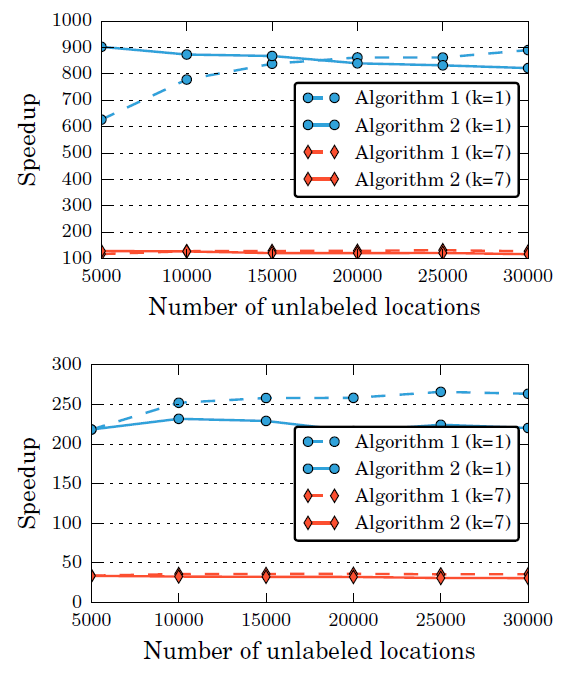
\includegraphics[width=0.8\linewidth]{cmp.png}
        \captionof{figure}{\color{Navy}Geodesic 1NN and 7NN with Algorithms \color{black} 2.1 \color{Navy}and \color{red}2.2\color{Navy}. (Top: 1600 labeled locations on 2m grid; Bottom: 400 labeled on 4m grid)}
    \end{center}


%----------------------------------------------------------------------------------------
%	APPLICATION
%----------------------------------------------------------------------------------------

\color{SaddleBrown} % SaddleBrown color for the conclusions to make them stand out

\section*{Applications}


\subsection*{Regressor Used}
    \normalsize
    \begin{itemize}
        \item K nearest neighbor regressor (KNN)
        \item Geodesic KNN (GNN)
        \item Semi-supervised Laplacian regressor
    \end{itemize}
    
\subsection*{Indoor Localization Using Wi-Fi Signals}
    \normalsize
    \begin{center}
        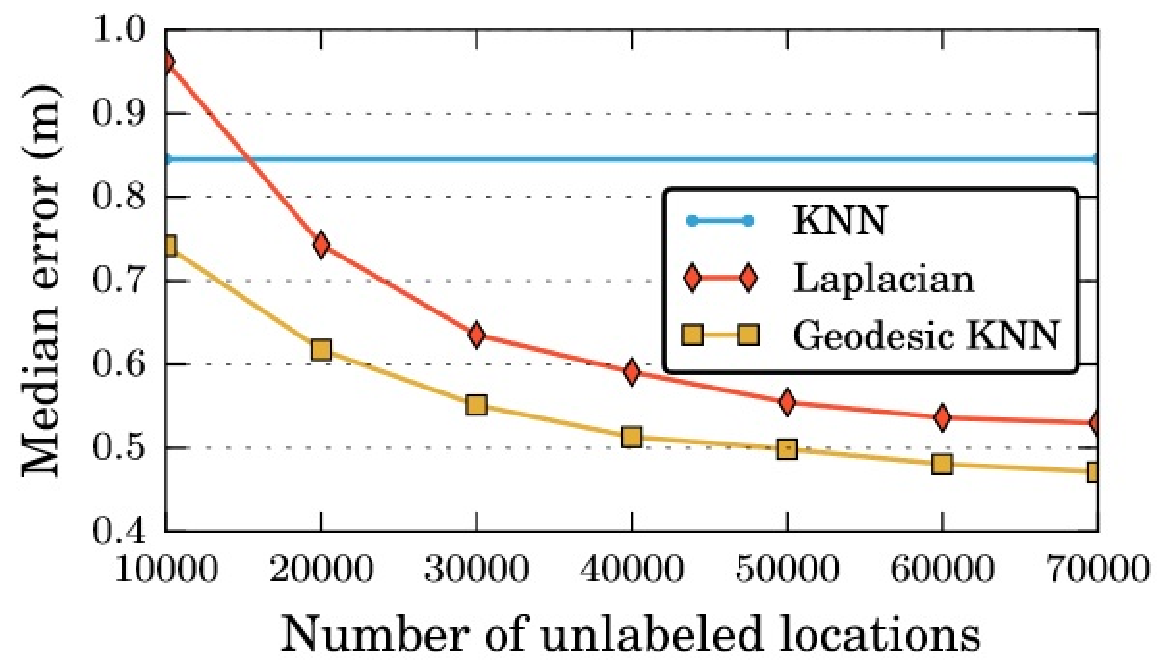
\includegraphics[width=0.8\linewidth]{simulatedacccase1-converted.pdf}
        \captionof{figure}{\color{SaddleBrown} Median localization error vs. number of unlabeled points with 1600 labeled points placed on a regular simulated grid with a side length of 2m. \cite{mainpaper}}
    \end{center}
    
    \begin{center}
        \begin{tabular}{l l l l l}
        \toprule
        \textbf{Labeled grid} & \textbf{n} & \textbf{kNN} & \textbf{GNN} & \textbf{Laplacian}\\
        \midrule
        1.5m & 73 & 1.49m & \textit{1.11}m & 1.36m \\
        2.0m & 48 & 2.27m & \textit{1,49}m & 1.65m \\
        3.0m & 23 & 3.41m & \textit{2.41}m & 2.79m \\
        \bottomrule
        \end{tabular}
    \captionof{table}{\color{SaddleBrown} Mean accuracy of kNN, geodesic kNN and Laplacian eigenbasis regression on the real data set. \cite{mainpaper}}
    \end{center}
    
    \begin{center}
        \begin{tabular}{l l l l}
        \toprule
        \textbf{\#unlabeled} & \textbf{GNN} & \textbf{Laplacian} & \textbf{graph build}\\
        \midrule
        1000 & 2.3s & 7.6s & 9s \\
        10000 & 7s & 195s & 76s \\
        100000 & 56s & 114min & 66min \\
        \bottomrule
        \end{tabular}
    \captionof{table}{\color{SaddleBrown} Runtime of Geodesic 7-NN vs. time to com-pute Laplacian eigenvectors. \cite{mainpaper}}
    \end{center}
    
\subsection*{Facial Pose Estimation}
    \normalsize
    \begin{center}
        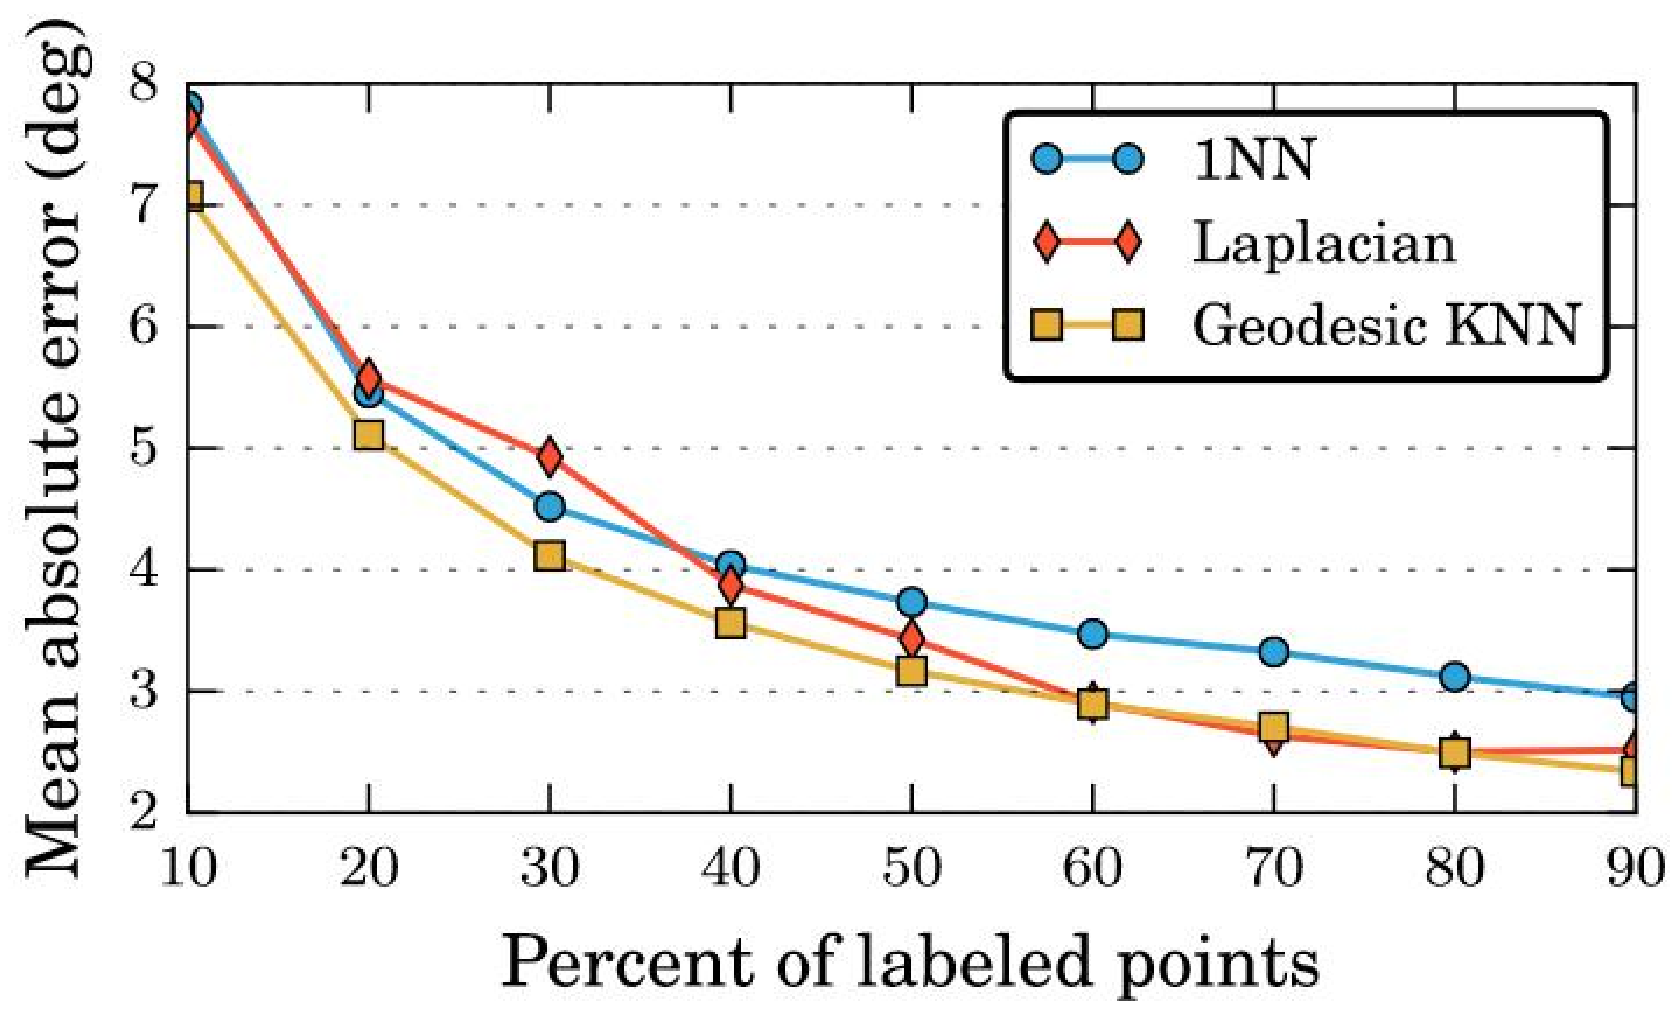
\includegraphics[width=0.8\linewidth]{case2-converted.pdf}
        \captionof{figure}{\color{SaddleBrown} Mean prediction error for the left-rightangle of the face. \cite{mainpaper}}
    \end{center}

\color{DarkSlateGray} % Set the color back to DarkSlateGray for the rest of the content

%----------------------------------------------------------------------------------------
%	REFERENCES
%----------------------------------------------------------------------------------------

\nocite{*} % Print all references regardless of whether they were cited in the poster or not
\bibliographystyle{plain} % Plain referencing style
\bibliography{sample} % Use the example bibliography file sample.bib

%----------------------------------------------------------------------------------------
%	ACKNOWLEDGEMENTS
%----------------------------------------------------------------------------------------

\section*{Acknowledgements}
We would like to thank Amit Moscovich, Ariel Jaffe, and Boaz Nadler for methodology, algorithm, and empirical results provided in ``Minimax-optimal semi-supervised regression on unknown manifolds''.

%----------------------------------------------------------------------------------------

\end{multicols}
\end{document}